\section{Background}

Throughout the paper, we use the notation $[L]$ to represent the set $\{1,\ldots, L\}$. We denote a sequence of tokens as $\vx = (x^1,\ldots,x^d) \in \gV^d$, where $d$ is the sequence length and $\gV := [V]$ is the vocabulary. Given our focus on masked diffusion models, we assume that the vocabulary includes a special mask token $\mask$. %

\subsection{Masked Diffusion Models}
\label{sec:back_mdm}
We focus on masked diffusion models (MDMs) \citep{llada2025}, deferring a more general introduction to discrete diffusion to Appendix~\ref{sec:appendix_extended_background}.
\paragraph{Training} MDMs learn to generate data by training a BERT-style \citep{devlin2019bert} masked predictor to reverse the forward noising process. Concretely, given a training sample $\vx_0 \sim p_{\text{data}}$, the forward process corrupts each token independently by setting it to the mask token with probability proportional to the diffusion timestep $t \in [0, 1]$: 
\begin{align*}
    p_{t}(\vx_t \mid \vx_0) := \prod_{k=1}^d p_t(x_t^k \mid \vx_0), \quad \text{where} \quad
    p_t(x_t^k \mid \vx_0)
    :=
    \begin{cases}
        1 - t, & \text{if } x_t^k = x_0^k, \\
        t, & \text{if } x_t^k = \mask, \\
        0, & \text{otherwise.}
    \end{cases} 
\end{align*}
Recent work has shown that an MDM parametrized by $\theta$ can learn the reverse process by maximizing the following evidence lower bound (ELBO) \citep{ou2024your}, $\gL(\theta) \leq \mathbb{E}_{\vx_0 \sim p_\text{data}} [\log p_{\theta}(\vx_0)]$:
\begin{align}
\label{eq:mdm}
    \gL(\theta) := \mathbb{E}_{t \sim U[0,1], \vx_0 \sim p_{\text{data}}, \vx_t \sim p_t (\vx_t \mid \vx_0)} \bigg[ \frac{1}{t} \sum_{k=1}^d \mathbf{1}[ x_t^k = \mask] \log p_{\theta}(x_0^k | \vx_t)\bigg] \: ,
\end{align}
with $\mathbf{1}[\cdot]$ denoting the indicator function. %

\paragraph{Generation} When generating an answer for a given prompt $\vx$, MDMs start with a sequence of all-masked tokens $\vy_T := (\mask, \ldots, \mask)$, where $L :=  |\vy_T|$ is a pre-specified maximum answer length. Then, in each sampling step $t \in [T]$, the MDM outputs token distributions $p_{t}^k := p_{\theta}(y_0^k = \cdot \mid \vx, \vy_{t})$ for all token positions $k \in [L]$. Then, a sampling strategy decides which subset $\gU_t \subseteq \gM_{t}$ of the still-masked positions $\gM_{t} := \{k \in [L] \mid y_{t}^k = \mask\}$ to unmask. A new, partially unmasked/denoised answer $\vy_{t-1}$ is obtained via 
\begin{align}
\label{eq:mdm_sampling}
    y_{t-1}^k := \begin{cases}
        y \sim p_{t}^k, & \text{if } k \in \gU_t, \\
        y_{t}^k, & \text{otherwise.}
    \end{cases} 
\end{align}
The stochasticity of sampling $y \sim p_{t}^k$ depends on the dLLM temperature $\tau$, with higher temperatures leading to more diverse (but often lower quality) generations.
When evaluating dLLMs, it is common to set $\tau=0$ \citep{llada2025, fastdllm2025} to maximize performance, resembling greedy decoding in AR LLMs.
However, unlike for autoregressive LLMs, setting the temperature $\tau$ to 0 is not sufficient to completely determine the generation process.
The choice of sampling strategy\footnote{We use the terms \emph{sampling} and \emph{unmasking} interchangeably throughout this paper.} is also important, since different choices will produce different unmasking sets $\gU_t$.
This clearly affects the sampling \emph{efficiency}, since generating multiple tokens in parallel will yield a complete answer faster than if they were generated one at a time.
However, it may also affect the \emph{quality} of the samples, since different unmasking sets will yield different conditions $\vx_t$, thus affecting the predicted token distributions $p_t^k$.
The need to carefully balance efficiency and quality has thus drawn considerable attention to the development of optimal sampling techniques for dLLMs (see \Cref{sec:related}). %


\subsection{Heuristic Samplers}
\label{sec:back_heuristics}
\begin{wrapfigure}{r}{0.45\linewidth}
    \vspace{-40pt}
    \centering
    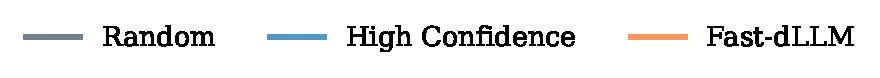
\includegraphics[width=\linewidth]{new_plots_nov4/legends/fig1a.pdf}
    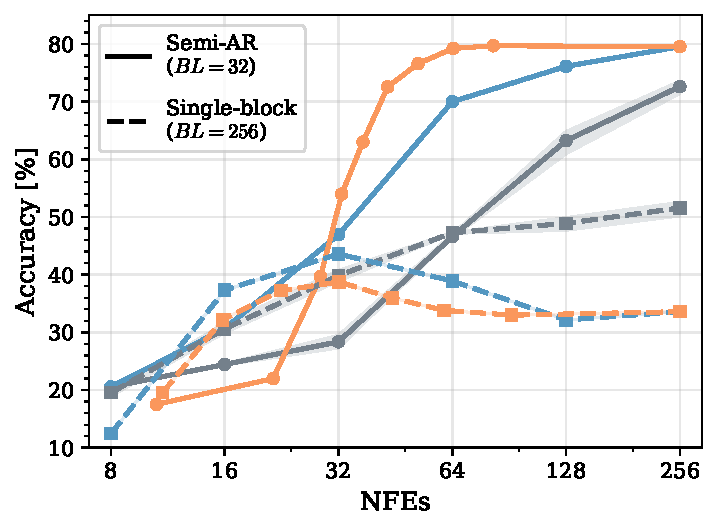
\includegraphics[width=\linewidth]{new_plots_nov4/fig1/simple-fig1-llada-gsm8k.pdf}
    \caption{LLaDA-8B-Instruct \citep{llada2025} on GSM8k, with semi-AR generation (8 blocks of $BL=32$; \protect\solidline) and without (one block of $BL=256$; \protect\dashedline). More datasets and models in Appendix \ref{sec:app-motivation}. Generation speed is measured in network function evaluations (NFEs), which corresponds to the number of sampling steps.} %
    \label{fig:motivation}
    \vspace{-10pt}
\end{wrapfigure}

One popular approach to decide which positions $\gU_t$ to unmask at each timestep is to construct a heuristic that leverages uncertainty measures derived from the predicted token distributions $p_t^k$ (\citealt{fastdllm2025, ben2025accelerated, wei2025accelerating, hong2025wide, li2025beyond, huang2025pc, kim2025train}; \emph{inter alia}). 
In particular, recent work has shown substantial efficiency gains by with heuristic strategies that employ the \emph{confidence} $c_{t}^k := \max_{v \in \gV} p_{t}^k(v)$ of the underlying dLLM in order to make their decisions. %
Two representative methods within this space
are \emph{high-confidence} unmasking \citep{chang2022maskgit},
in which each forward pass unmasks a fixed number of tokens ($K$) with the highest confidences, 
$$
\gU_t^{K} := \Big\{\underset{I \subseteq \gM_t,\ |I| = K}{\arg\max}\ \sum_{k \in I} c_t^k \Big\}
$$
as well as the confidence-thresholding strategy of Fast-dLLM \citep{fastdllm2025}, which allows for a variable number of tokens to be unmasked at each step by comparing the confidences to a fixed threshold $\lambda$:\footnote{Note that it is possible for no token confidence to exceed the pre-determined threshold $\lambda$.
In this case, \cite{fastdllm2025} propose to unmask the position with the highest confidence among the remaining masked tokens, to prevent the sampling from getting stuck.}
\begin{align*}
\gU_t^{\lambda} := \{ k \in \gM_t \mid c_t^k > \lambda \}.
\end{align*}
 Notably, \cite{fastdllm2025} showed that when combining confidence-thresholding sampling with additional optimizations such as KV-caching, dLLMs can live up to their promise and surpass AR models in token throughput, while maintaining comparable generation quality. Moreover, they provide theoretical justification for their sampling design by showing that sampling from high-confidence marginals closely approximates sampling from the joint distribution over token positions.

Despite the undeniable recent success of confidence-based samplers, relying on handcrafted solutions comes with certain drawbacks. Beyond the obvious need for careful design (e.g., selecting an appropriate confidence measure or threshold value $\lambda$), we also found that these methods often exhibit high sensitivity to the exact sampling configuration. For instance, many heuristics rely on semi-autoregressive (semi-AR) generation \citep{arriola2025block,llada2025}, where decoding proceeds one ``block'' of tokens at a time, with block length $BL$ serving as yet another hyperparameter. As shown in \autoref{fig:motivation}, outside this semi-AR regime, confidence-based heuristics can degrade to below-random performance and may no longer benefit from increased compute budgets (i.e., higher numbers of function evaluations, NFEs). These limitations raise a natural question whether effective sampling methods can be \textit{learned} rather than manually designed, which we explore next.



